\subsection{Specimen geometry}

The tested structure is a bulk resin test specimen according to DIN EN ISO 527-2 with geometry 1BA. The specimen geometry and its dimensions are shown in \autoref{fig:test_elastic-plastic_tensile_bulk_tension_dimensions} and \autoref{tab:AdhMatChar_ep_BulkTension_Dims}.

\begin{figure}[htbp]
\centering
\newlength{\figwidth}
\setlength{\figwidth}{0.6\linewidth}
\def\mlf{0.125}
\begin{tikzpicture}
  % Bild
  %\node[anchor=south west,inner sep=0pt] (probe) at (0,0){\includegraphics[width=.6\linewidth]{../../Material/Figures/Tension_Dogbone_Dimensions}};
  \node[anchor=south west,inner sep=0pt] (probe) at (0,0){\includegraphics[width=\figwidth]{Tension_Dogbone_Dimensions}};
  % Scope
  \begin{scope}[x={(probe.south east)},y={(probe.north west)}]
    % Symmetrie
    \def\x{0.2}
    \def\y{0.27}
    \draw[dashdotted] ($(probe.east)+( \x cm, 0)$) -- ($(probe.west)-( \x cm, 0)$);
    \draw[dashdotted] ($(probe.center)+( 0, \y)+( 0,\x cm)$) -- ($(probe.center)-( 0, \y)-( 0,\x cm)$);    
    % Masse
    % horizontal
    % up
    \def\df{1.0}
    % l1
    \def\ml{0.5}
    \def\x{0.2}
    \def\y{0.27}
    \draw ($(probe.center)+( \x, \y)$) -- ($(probe.center)+( \x, \y)+(0, \df*\ml cm)$);
    \draw ($(probe.center)+(-\x, \y)$) -- ($(probe.center)+(-\x, \y)+(0, \df*\ml cm)$);
    \draw[latex-latex] ($(probe.center)+( \x, \y)+(0, \df*\ml cm)-(0,\df*\mlf cm)$) -- ($(probe.center)+(-\x, \y)+(0, \df*\ml cm)-(0,\df*\mlf cm)$) node [midway, above] {$l_1$};
    % l2
    \def\ml{0.75}
    \def\x{0.345}
    \def\y{0.52}
    \draw ($(probe.center)+( \x, \y)$) -- ($(probe.center)+( \x, \y)+(0, \df*\ml cm)$);
    \draw ($(probe.center)+(-\x, \y)$) -- ($(probe.center)+(-\x, \y)+(0, \df*\ml cm)$);
    \draw[latex-latex] ($(probe.center)+( \x, \y)+(0, \df*\ml cm)-(0,\df*\mlf cm)$) -- ($(probe.center)+(-\x, \y)+(0, \df*\ml cm)-(0,\df*\mlf cm)$) node [midway, above] {$l_2$};
    % t
    \def\xo{-0.4175}	% the right
    \def\xt{-0.444}	% the left
    \draw ($(probe.center)+( \xo, \y)$) -- ($(probe.center)+( \xo, \y)+(0, \df*\ml cm)$);
    \draw ($(probe.center)+( \xt, \y)$) -- ($(probe.center)+( \xt, \y)+(0, \df*\ml cm)$);
    \draw[arrows={latex[reversed]-latex[reversed]}] ($(probe.center)+( \xo, \y)+(0, \df*\ml cm)+(0.125cm,-\df*\mlf cm)$) -- ($(probe.center)+( \xt, \y)+(0, \df*\ml cm)-(0.125cm,\df*\mlf cm)$) node [midway, above] {$t$};
    \draw ($(probe.center)+( \xo, \y)+(0, \df*\ml cm)+(0.25cm,-\df*\mlf cm)$) -- ($(probe.center)+( \xt, \y)+(0, \df*\ml cm)-(0.25cm,\df*\mlf cm)$);
    % l3
    \def\ml{1.35}
    \def\x{0.50}
    \def\y{0.52}
    \draw ($(probe.center)+( \x, \y)$) -- ($(probe.center)+( \x, \y)+(0, \df*\ml cm)$);
    \draw ($(probe.center)+(-\x, \y)$) -- ($(probe.center)+(-\x, \y)+(0, \df*\ml cm)$);
    \draw[latex-latex] ($(probe.center)+( \x, \y)+(0, \df*\ml cm)-(0,\df*\mlf cm)$) -- ($(probe.center)+(-\x, \y)+(0, \df*\ml cm)-(0,\df*\mlf cm)$) node [midway, above] {$l_3$};
    % down
    \def\df{-1.0}
    % L0
    \def\ml{0.5}
    \def\x{0.175}
    \def\y{-0.27}
    \draw ($(probe.center)+( \x, \y)$) -- ($(probe.center)+( \x, \y)+(0, \df*\ml cm)$);
    \draw ($(probe.center)+(-\x, \y)$) -- ($(probe.center)+(-\x, \y)+(0, \df*\ml cm)$);
    \draw[latex-latex] ($(probe.center)+( \x, \y)+(0, \df*\ml cm)-(0,\df*\mlf cm)$) -- ($(probe.center)+(-\x, \y)+(0, \df*\ml cm)-(0,\df*\mlf cm)$) node [midway, below] {$L_0$};
    % L
    \def\ml{0.75}
    \def\x{0.38}
    \def\y{-0.52}
    \draw ($(probe.center)+( \x, \y)$) -- ($(probe.center)+( \x, \y)+(0, \df*\ml cm)$);
    \draw ($(probe.center)+(-\x, \y)$) -- ($(probe.center)+(-\x, \y)+(0, \df*\ml cm)$);
    \draw[latex-latex] ($(probe.center)+( \x, \y)+(0, \df*\ml cm)-(0,\df*\mlf cm)$) -- ($(probe.center)+(-\x, \y)+(0, \df*\ml cm)-(0,\df*\mlf cm)$) node [midway, below] {$L$};
    % vertical
    % right
    \def\df{1.0}
    % b1
    \def\ml{0.5}
    \def\x{0.5075}
    \def\y{0.25}
    \draw[dashed] ($(probe.center)+( 0.3, \y)$) -- ($(probe.center)+( \x, \y)$);
    \draw[dashed] ($(probe.center)+( 0.3,-\y)$) -- ($(probe.center)+( \x,-\y)$);
    \draw ($(probe.center)+( \x, \y)$) -- ($(probe.center)+( \x, \y)+(\df*\ml cm, 0)$);
    \draw ($(probe.center)+( \x,-\y)$) -- ($(probe.center)+( \x,-\y)+(\df*\ml cm, 0)$);
    \draw[latex-latex] ($(probe.center)+( \x, \y)+(\df*\ml cm,0)-(\df*\mlf cm,0)$) -- ($(probe.center)+( \x,-\y)+( \df*\ml cm,0)-(\df*\mlf cm,0)$) node [midway, right] {$b_1$};
    % left
    \def\df{-1.0}
    % b2
    \def\ml{0.5}
    \def\x{-0.5075}
    \def\y{0.5}
    \draw ($(probe.center)+( \x, \y)$) -- ($(probe.center)+( \x, \y)+(\df*\ml cm, 0)$);
    \draw ($(probe.center)+( \x,-\y)$) -- ($(probe.center)+( \x,-\y)+(\df*\ml cm, 0)$);
    \draw[latex-latex] ($(probe.center)+( \x, \y)+(\df*\ml cm,0)-(\df*\mlf cm,0)$) -- ($(probe.center)+( \x,-\y)+( \df*\ml cm,0)-(\df*\mlf cm,0)$) node [midway, left] {$b_2$};
    %
    % Radius
    \def\x{0.2}
    %\draw[-latex] ($(probe.center)+(\x,-2.9)$) node[cross out,draw=black,rotate=45,dashdotted,inner sep=0pt,outer sep=0pt,minimum size=0.5cm]{} -- ($(probe.center)+(1.5*\x,-0.375)$) node [midway, above, sloped] {$r$};
    %\draw[-latex] ($(probe.center)+(\x,-2.9)$) -- ($(probe.center)+(1.5*\x,-0.375)$) node [midway, above, sloped] {$r$};
    \draw[-latex] ($(probe.center)+(1.375*\x,-0.8)$) -- ($(probe.center)+(1.5*\x,-0.375)$) node [midway, above, sloped] {$r$};
    % Koordinatensystem
    % Origin
    \coordinate (origin) at (0.0,-0.5);
    \draw[-latex] (origin.center) -- ($(origin.center)+(0.4cm,0)$) node [anchor=north west,xshift=-0.5em,yshift=0.25ex] {$x$};
    \draw[-latex] (origin.center) -- ($(origin.center)+(0,0.4cm)$) node [anchor=north east,xshift= 0.25ex,yshift= 0.5em] {$y$};
%     \draw ($(probe.center)+(-\x, \y)$) -- ($(probe.center)+(-\x, \y)+(0, \df*\ml cm)$);
%     \draw[latex-latex] ($(probe.center)+( \x, \y)+(0, \df*\ml cm)-(0,\df*\mlf cm)$) -- ($(probe.center)+(-\x, \y)+(0, \df*\ml cm)-(0,\df*\mlf cm)$) node [midway, below] {$L$};
  \end{scope}
\end{tikzpicture}
\caption{Bulk tension test dimensions [DIN EN ISO 527-2, 2012]}
\label{fig:test_elastic-plastic_tensile_bulk_tension_dimensions}
\end{figure}

\begin{table}[htbp]
\begin{tabularx}{\linewidth}{%
 c%
 X%
 c%
 S[table-format=3.1,table-figures-uncertainty=1]
%  S[table-format=3.1,table-figures-uncertainty=1]
%  S[table-format=3.1,table-figures-uncertainty=1]
%  S[table-format=3.1,table-figures-uncertainty=1]
 S[table-format=3.1]
}
\toprule
% &&&\multicolumn{4}{c}{Specimen type}	\\
\multicolumn{2}{c}{Variable \& Description} & Unit & {Standard}	& {Model \& Test}\\
\midrule
$l_3$	& Overall length				& $\si{\milli\meter}$	& {$\ge\num{75}$}	& 75	\\
$l_1$	& Parallel narrow length			& $\si{\milli\meter}$	& 30\pm0.5		& 30	\\
$r$	& Radius					& $\si{\milli\meter}$	& {$\ge\num{30}$}	& 40.45	\\
$l_2$	& Distance between wide parallel edges		& $\si{\milli\meter}$	& 58\pm2		& 58	\\
$b_2$	& Wide parallel edge width			& $\si{\milli\meter}$	& 10\pm0.5		& 10	\\
$b_1$	& Narrow parallel edge width			& $\si{\milli\meter}$	& 5\pm0.5		& 5	\\
$t$	& Preferred thickness				& $\si{\milli\meter}$	& {$\ge\num{2}$}	& 2	\\
% \multirow{2}{*}{$L_0$}	& Measuring length (Preferred)	& $\si{\milli\meter}$	& 25\pm0.5	\\
% & Measuring length (Quality control)			& $\si{\milli\meter}$	& 50\pm0.5	\\
$L_0$	& Measuring length				& $\si{\milli\meter}$	& 25\pm0.5		& 25	\\
$L$	& Clamp distance				& $\si{\milli\meter}$	& {${l_2}_{\hphantom{\pm}0}^{+2}$}	& 58	\\
\bottomrule
\end{tabularx}
\caption{Bulk tensile dimensions for test specimen 1BA [DIN EN ISO 527-2, 2012]}
\label{tab:AdhMatChar_ep_BulkTension_Dims}
\end{table}

The load-displacement curves are measured using strain gauges on one side of the specimen. The resulting unsymmetrical behavior in the area of the strain gauge in combination with the localised change in stiffness in this area leads to failure in the area of the strain gauge.
% Messung einseitig mit DMS -> Unsymmetrie+Kerbwirkung des DMS+Steifigkeit gegen�ber dem Reinharz f�hrt zuverl�ssig zu Versagen an ``Kanten'' des DMS